
\section{Cycle Benchmarking}
\label{sec:cb}
We used the cycle benchmarking protocol studied in \cite{Erhard2019} and TrueQ software developed by Quantum Benchmark.



\subsection{Cycle Benchmarking Procedure?}
The measured process infidelities ($e_F$) obtained using CB protocol are presented in 


The cycle benchmarking data was obtained using the following variables. For each cycle of interest we used sequence lengths of 2, 10, and 22, respectively. The sequence length refers to the number of times the cycle of interest appears apart from state inversion. The number of random circuits used in each sequence length is 48. Each of these circuits at each sequence length were run $N_\text{shots}=128$ times. 

The process infidelity is estimated from the average value of the individual Pauli infidelities.


\subsubsection{Process Infidelity Measurements}
The process infidelity ($e_{F}$) was calculated using cycle benchmarking method for CNOT cycles seen in Fig.~\ref{fig:BoeblingenCycles}. Each row in Fig.~\ref{fig:BoeblingenCycles} corresponds to the CNOT cycles  studied for each qubit layout. There are four cycles studied for each qubit layout and we label each of these unique cycle as cycle 1, cycle 2, cycle 3 and cycle 4, respectively from left to right.
\begin{figure}[ht!]
    % \centering
    % \includegraphics[width=2.2\columnwidth]{final_plot.pdf}
    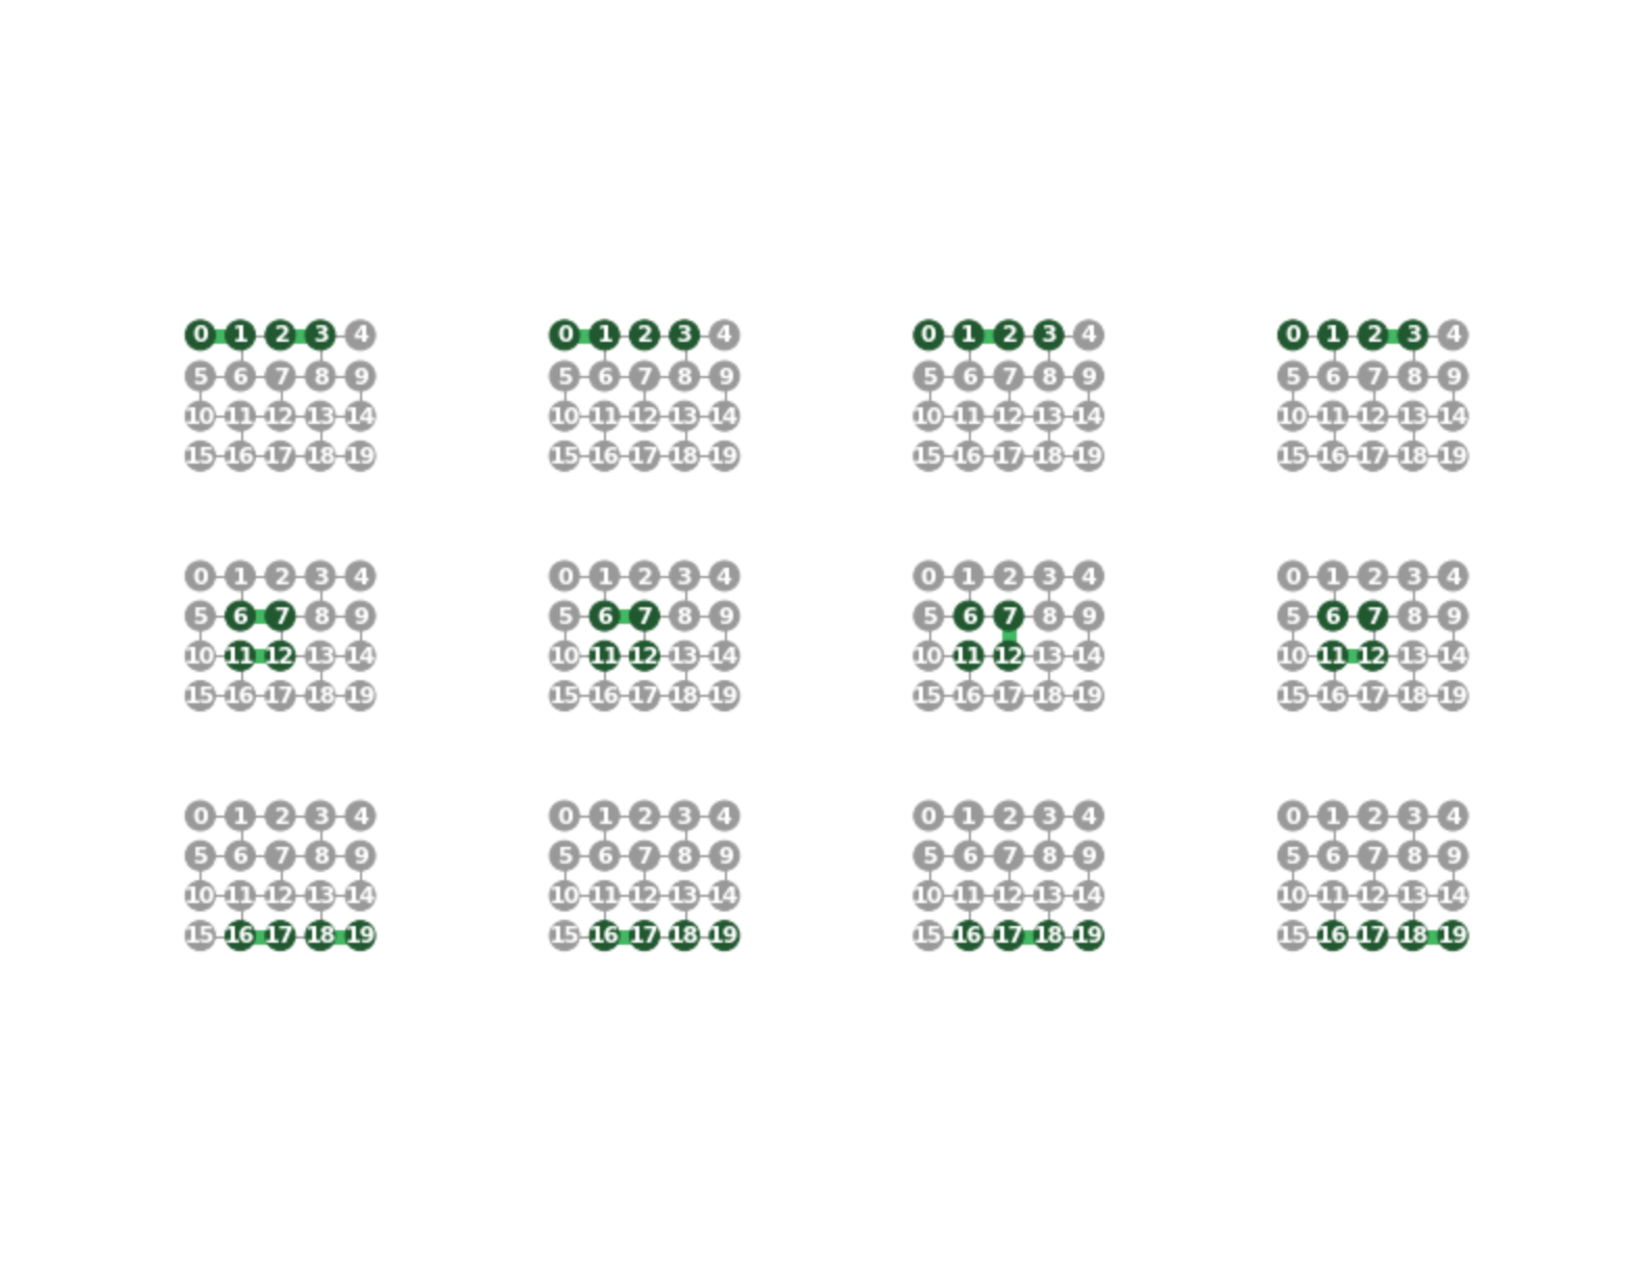
\includegraphics[scale=0.4]{BoeblingenCycles.pdf}
    \caption{The CNOT cycles used to calculate the process infidelities on IBM Q Boeblingen device.}
    \label{fig:BoeblingenCycles}
\end{figure}






\subsubsection{Quantum Capacity (QCap) Bound}
In Fig.s~\ref{fig:QCapCirc1}, \ref{fig:QCapCirc2}, \ref{fig:QCapCirc1and2} we present the QCap bound ($e_{IU}$) values calculated as a function of number of Trotter steps for circuits 1, circuit 2 and circuits 1 and 2 together. The data in Fig.~\ref{fig:QCapCirc1} demonstrates that qubit layout [6, 7, 12, 11] on Boeblingen quantum hardware performs the best for almost all runs and in each day of the experiment for Circuit 1. 

We also studied quantum capacity (QCap) as a function of the number of Trotter steps. QCap is able to estimate an upper bound on the total variational distance (TVD) without a full quantum simulation by characterizing the error rate of each cycle in the circuit and combining the results. This upper bound assumes the circuit is being run under randomized compiling (RC). Under RC, each dressed cycle of a circuit will have a stochastic error model whose process fidelity is estimated directly by CB. In this setting, errors accumulate in a circuit in a predictable way: the process fidelity of the circuit is the product of the process fidelity of each cycle. This parameter is estimated as this product, with error bars derived from standard propagation of uncertainty techniques. {\color{red}{KYA: Cite QB website.}}

We conducted QCap measurements for two quantum circuits as seen in Fig.~\ref{fig:IsingTrotterCircs}. Both of these quantum circuits result in time evolution of a state with $\mathcal{U}=e^{-iH_{\text{OBC}}\tau}$ using Trotterization where $\tau$ is the time interval for one Trotter step.  
\begin{figure*}[!tb]
\[ {\Qcircuit @C=0.5em @R=0.5em {
     \lstick{} & \gate{R_Z(h \tau)} & \multigate{1}{R_{XX}(2 J \tau)} &\qw&\qw  & & & &\\ 
     \lstick{} & \gate{R_Z(h \tau)}  & \ghost{R_{XX}(2 J \tau)} & \multigate{1}{R_{XX}(2 J \tau)}&\qw & & & &\\
     \lstick{} &  \gate{R_Z(h \tau)} & \multigate{1}{R_{XX}(2 J \tau)}&\ghost{R_{XX}(2 J \tau)}&\qw & & & & \\
     \lstick{} &  \gate{R_Z(h \tau)} & \ghost{R_{XX}(2 J \tau)} &\qw&\qw& & & &}}
    { \Qcircuit @C=0.5em @R=0.5em {
     \lstick{} & \gate{R_Z(h \tau)} & \multigate{1}{R_{XX}(2 J \tau)} &\qw&\qw &\qw & \qw\\ 
     \lstick{} & \gate{R_Z(h \tau)}  & \ghost{R_{XX}(2 J \tau)} & \multigate{1}{R_{XX}(2 J \tau)}&\qw&\qw&\qw \\
     \lstick{} &  \gate{R_Z(h \tau)} & \qw&\ghost{R_{XX}(2 J \tau)}&\qw & \multigate{1}{R_{XX}(2 J \tau)}\\
     \lstick{} &  \gate{R_Z(h \tau)} & \qw &\qw&\qw&\ghost{R_{XX}(2 J \tau)}}
}\]
\caption{The quantum circuit for one Trotter step of the time evolution with the open boundary condition Ising model Hamiltonian. We define the quantum circuit in left (right) panel as Circuit 1 (Circuit 2).}
\label{fig:IsingTrotterCircs}
\end{figure*}



\begin{figure*}[ht!]
    % \centering
    % \includegraphics[width=2.2\columnwidth]{final_plot.pdf}
    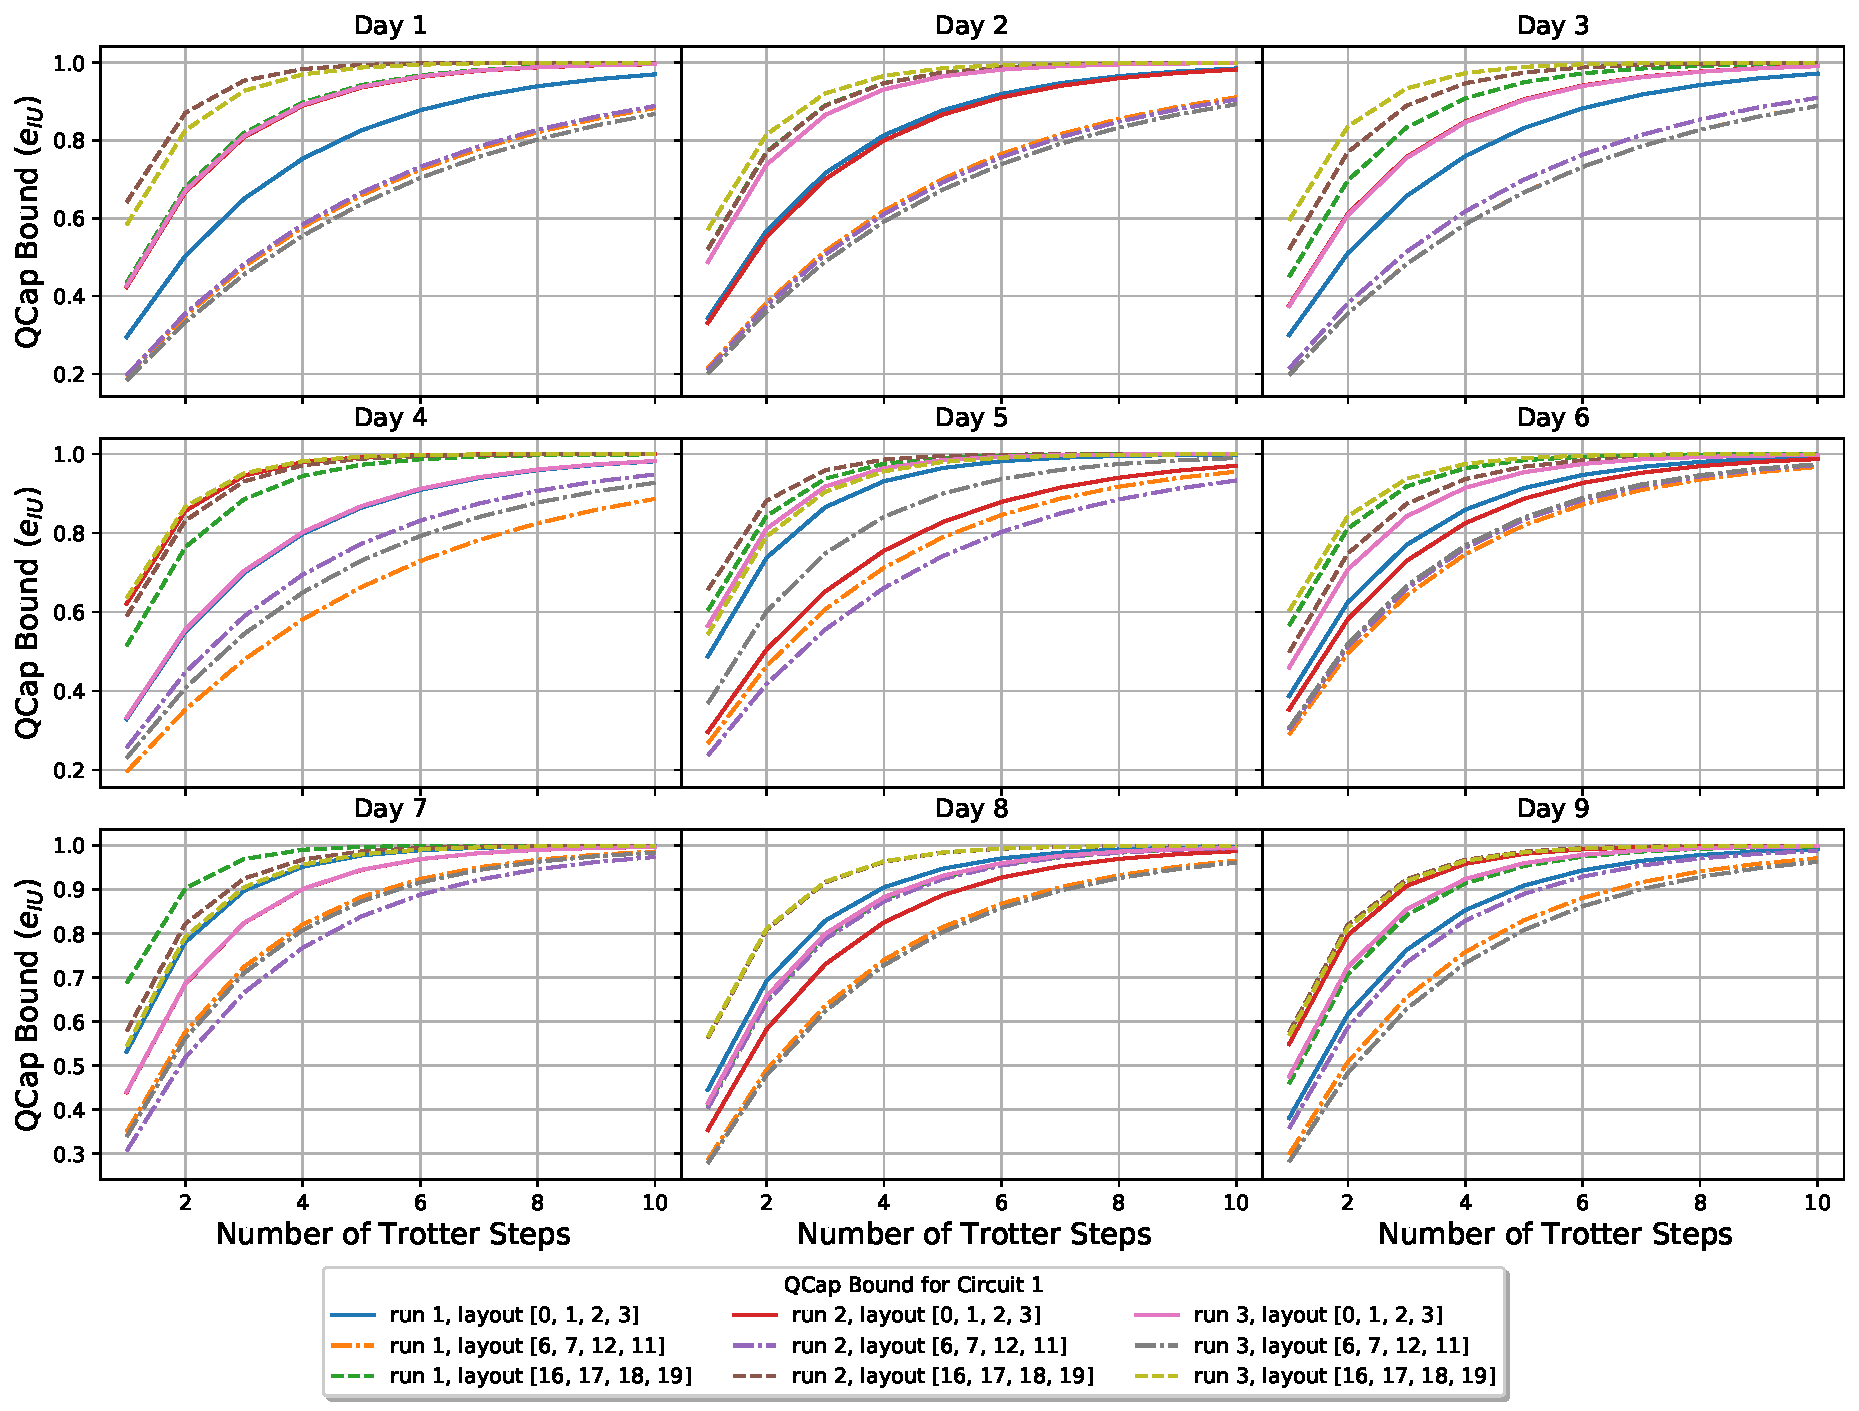
\includegraphics[scale=0.5]{QCapBoundForEachDay_Circ1.pdf}
    \caption{QCap bounds calculated using IBM Q Boeblingen hardware as a function of number of Trotter steps for circuit 1, layouts $[0,1,2,3],[6,7,12,11],[16,17,18,19]$, runs 1, 2, and 3 between days 01/23-31/2021 are presented.}
    \label{fig:QCapCirc1}
\end{figure*}
\begin{figure*}[ht!]
    % \centering
    % \includegraphics[width=2.2\columnwidth]{final_plot.pdf}
    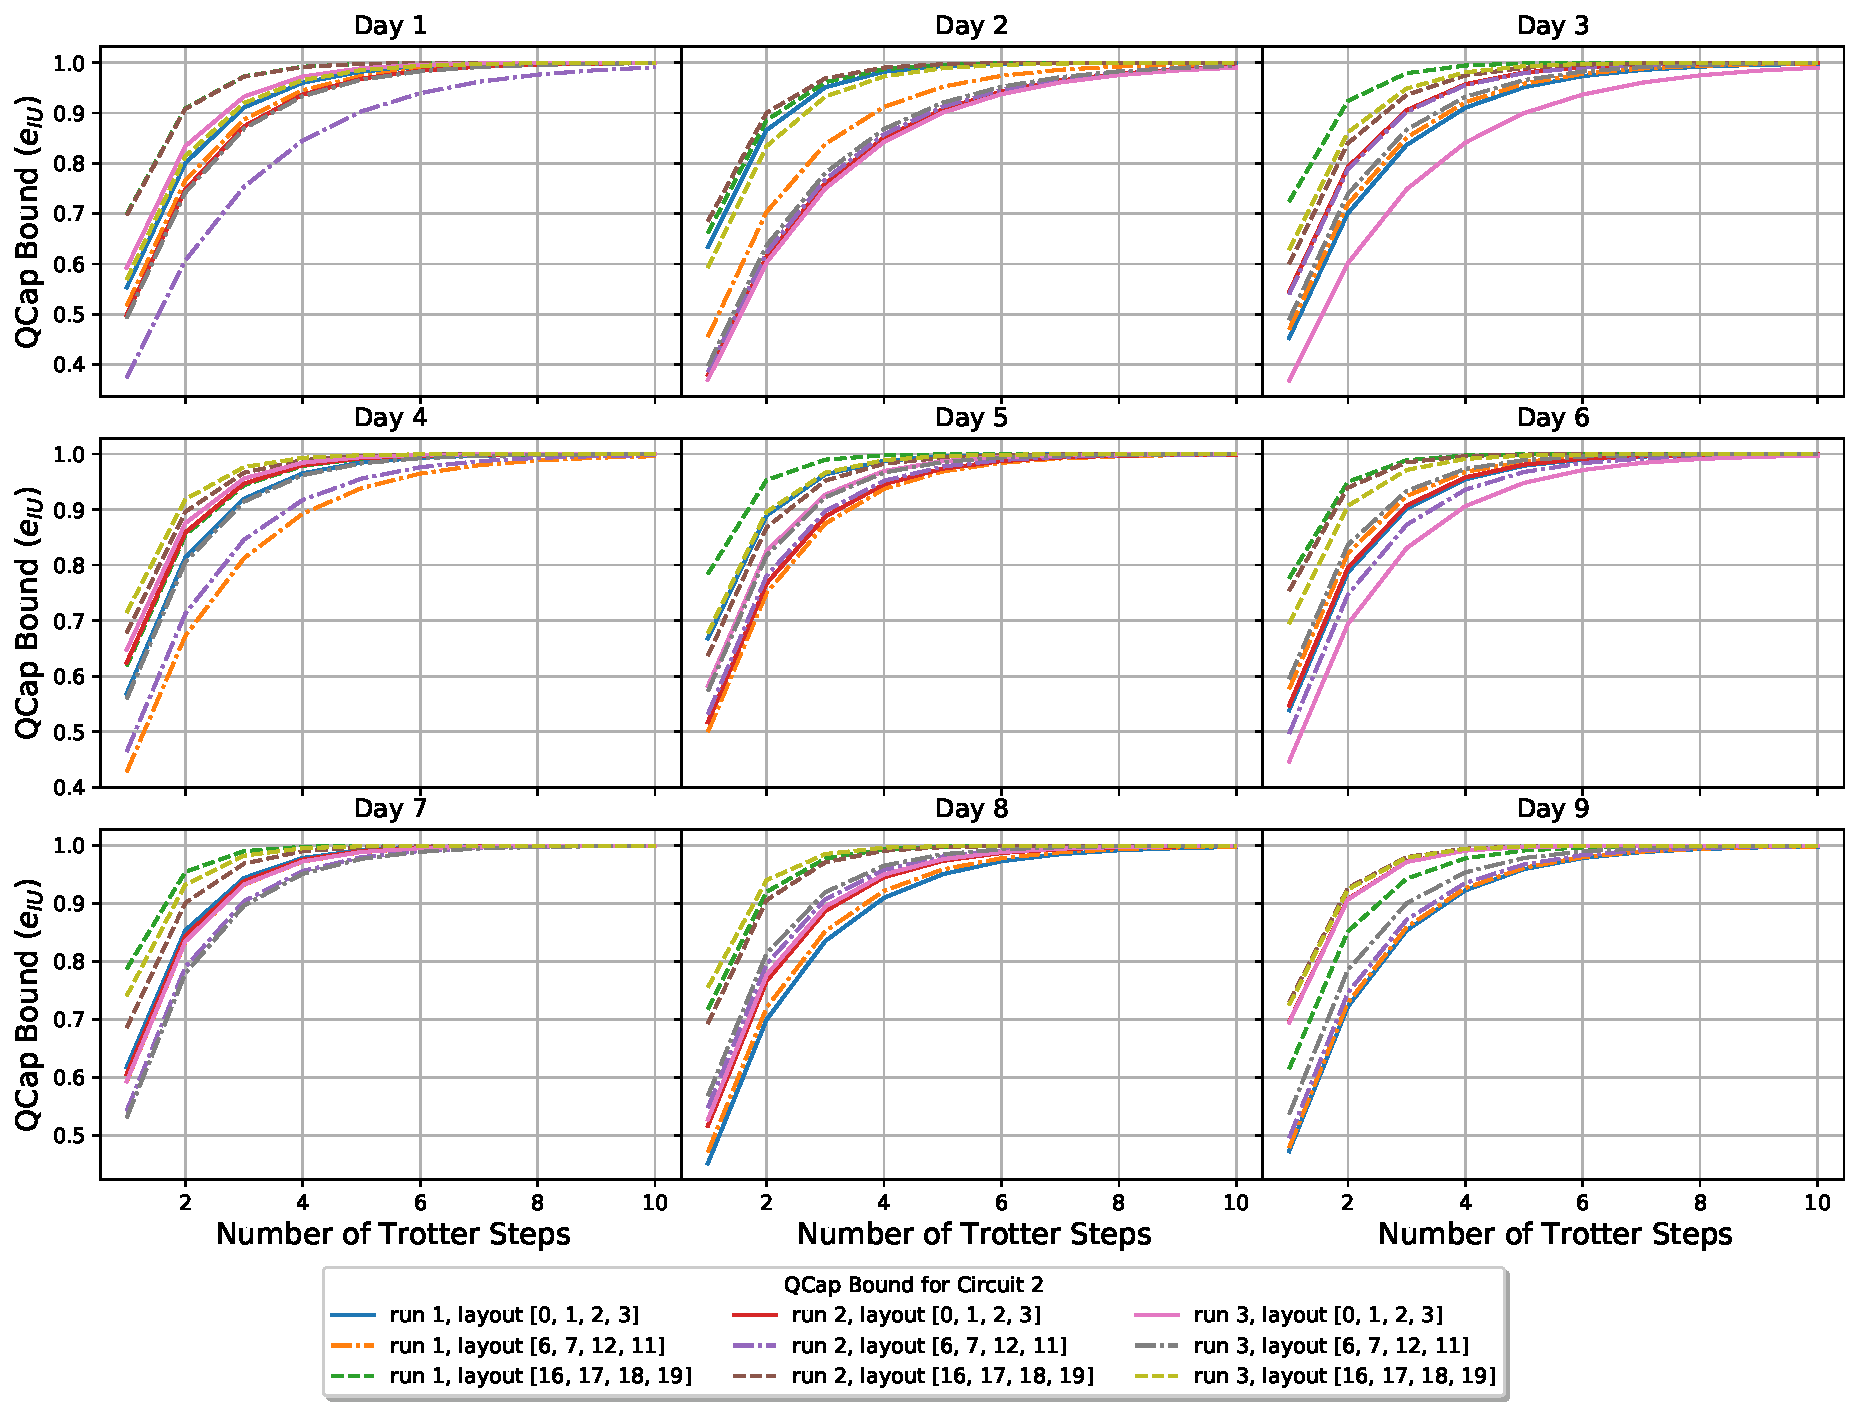
\includegraphics[scale=0.5]{QCapBoundForEachDay_Circ2.pdf}
    \caption{QCap bounds calculated using IBM Q Boeblingen hardware as a function of Trotter steps for circuit 2, layouts $[0,1,2,3],[6,7,12,11],[16,17,18,19]$, runs 1, 2, and 3 between days 01/23-31/2021 are presented.}
    \label{fig:QCapCirc2}
\end{figure*}

\begin{figure*}[ht!]
    % \centering
    % \includegraphics[width=2.2\columnwidth]{final_plot.pdf}
    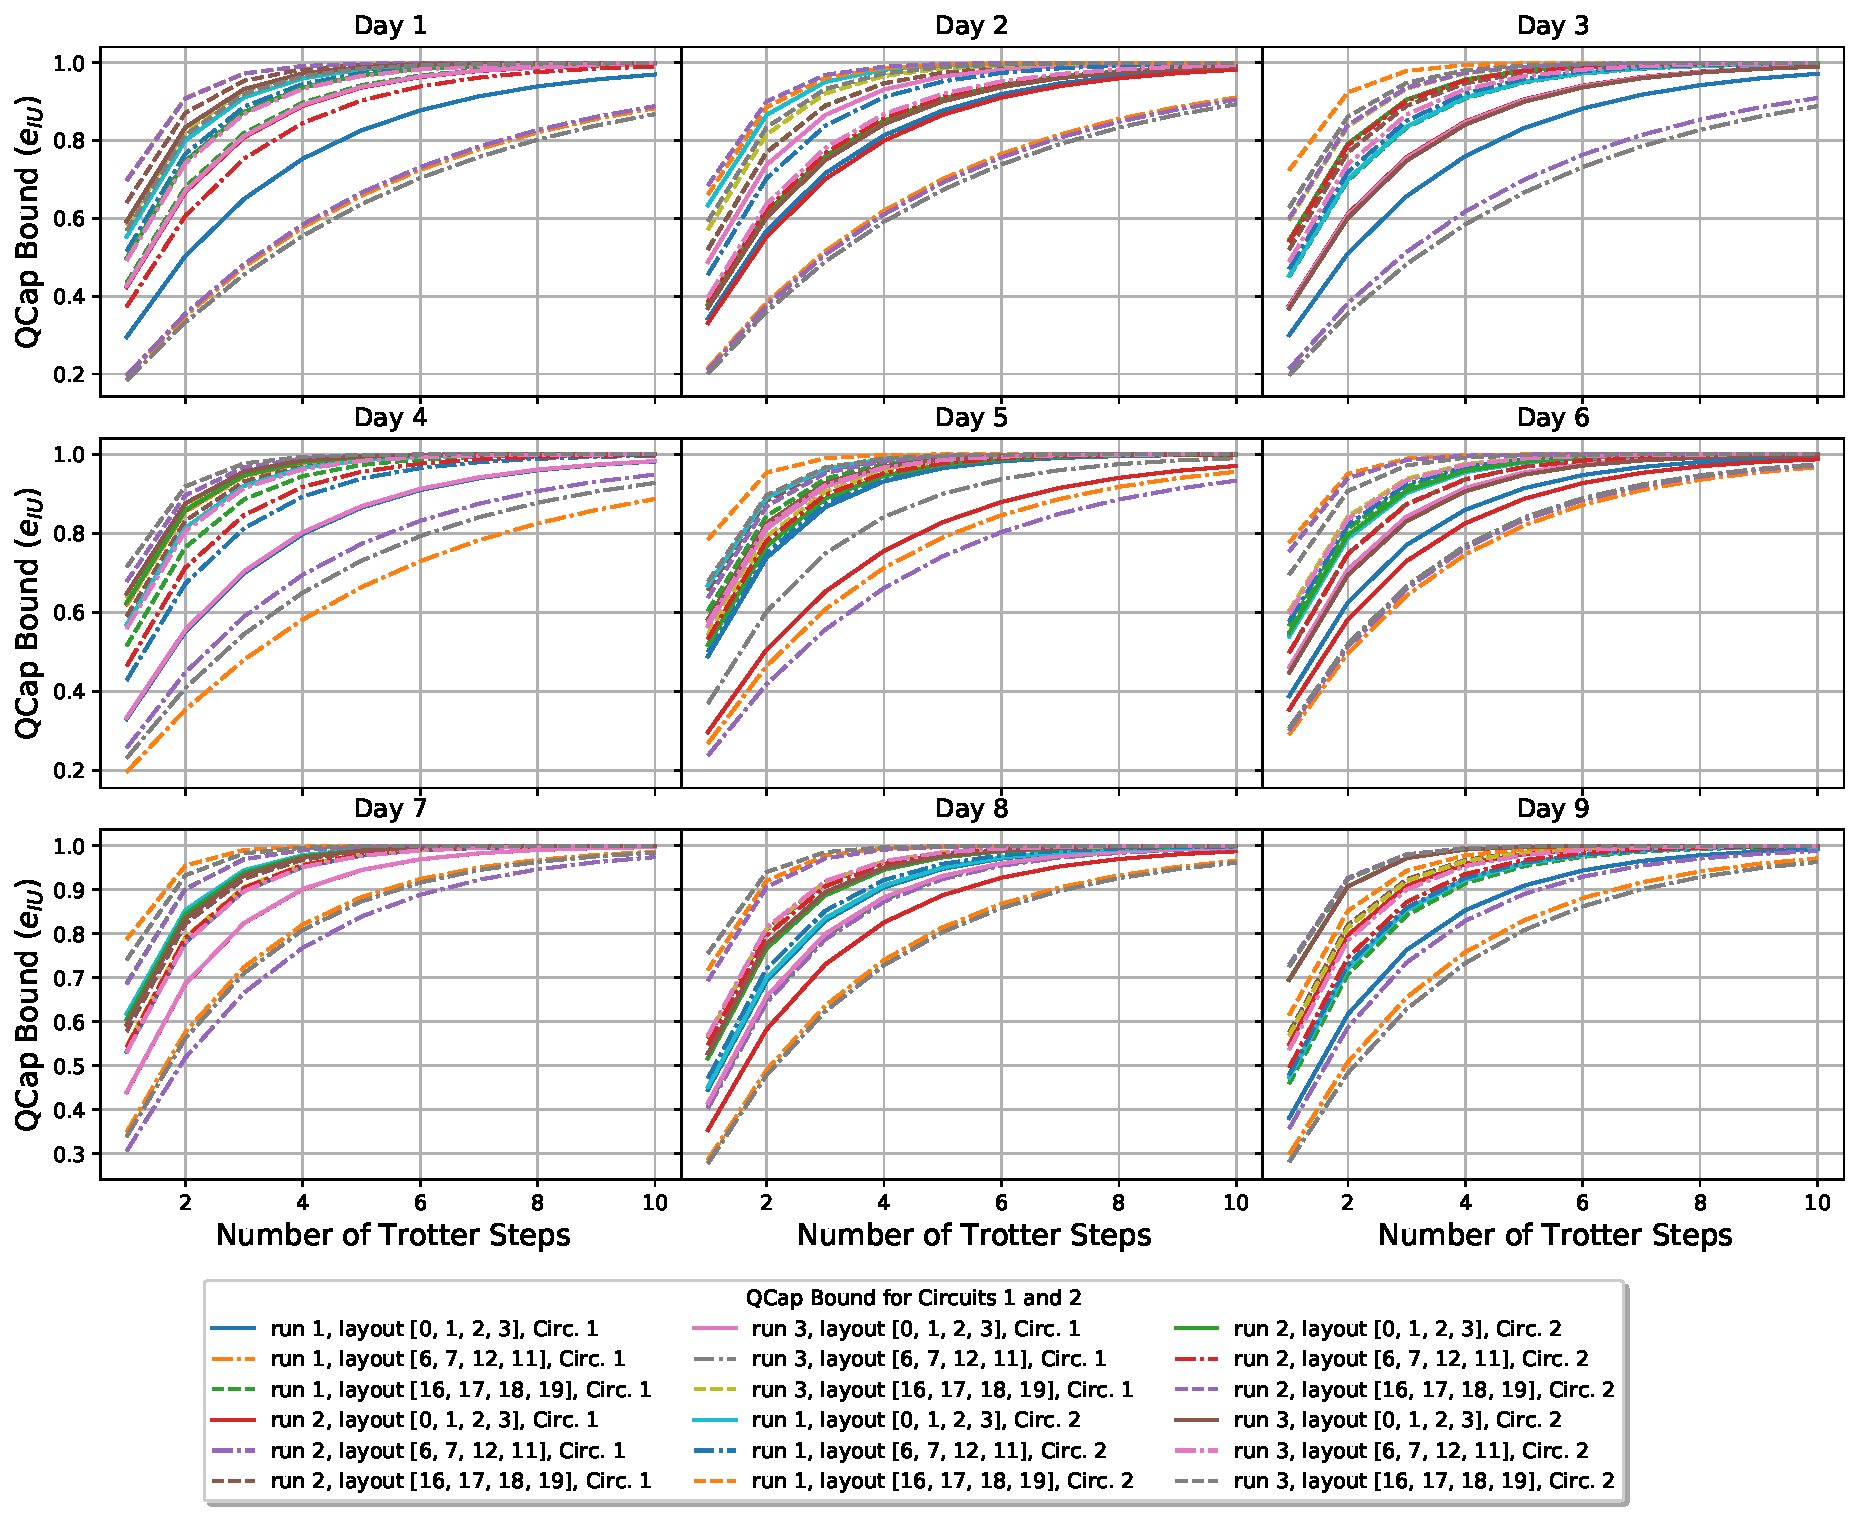
\includegraphics[scale=0.5]{QCapBoundForEachDay_Circ1andCirc2.pdf}
    \caption{QCap bounds calculated using IBM Q Boeblingen hardware as a function of number of Trotter steps for circuit 1 and 2 are compared for layouts $[0,1,2,3],[6,7,12,11],[16,17,18,19]$, runs 1, 2, and 3 between days 01/23-31/2021 are presented.}
    \label{fig:QCapCirc1and2}
\end{figure*}

The parameters used for QCap measurements is as follows. Due to limited access to the dedicated mode on Boeblingen device we use sequence lengths of 4 and 16. The number of random circuits in this case is 30 and each of these circuits were run $N_{\text{shots}}=128$. 

